%Template v.1.0: Taylor Arnold and Simon Gabay, december 2025
% CECI EST UN FICHIER DE MODÈLE LATEX POUR LES ARTICLES INCLUS DANS
% *Anthology of Computers and the Humanities*. AJOUTEZ L'OPTION
% 'final' LORS DE LA CRÉATION DE LA VERSION FINALE DE L'ARTICLE. 
% NE PAS modifier la classe du document
%\documentclass[final, fra, custom]{anthology-ch}     % pour la version finale
\documentclass[final, fra]{anthology-ch}      % pour la soumission

% CHARGER LES PACKAGES LaTeX
\usepackage{booktabs}
\usepackage{graphicx}

% AJOUTEZ vos propres packages avec \usepackage{}
\usepackage{tabularx}
\usepackage{tikz}
\usepackage{wrapfig}
\usetikzlibrary{positioning}

% TITRE DE LA SOUMISSION
% Remplacez ceci par le titre de votre soumission
\title{Structuration argumentative des débats parlementaires par IA : vers une modélisation interprétable des dynamiques discursives}

% INFORMATIONS SUR LES AUTEURS ET LES AFFILIATIONS
% Pour chaque auteur, utilisez une nouvelle commande \author, avec
% les numéros entre crochets indiquant les affiliations correspondantes
% (section suivante) et l'ORCID-ID pour chaque auteur.  
\author[1]{Adam Faci}[
  orcid=0000-0001-7216-9487,
  email=adam.faci@huma-num.fr
]


\affiliation{1}{Huma-Num IR* (UAR 3598), CNRS, Paris, France}

% Il doit y avoir un appel à \affiliation pour chaque affiliation des auteurs.
% Plusieurs affiliations peuvent être attribuées à un auteu
% MOTS-CLÉS
% Fournissez un ou plusieurs mots-clés séparés par des virgules
% en utilisant les commandes suivantes
\keywords[fra]{grands modèles de langage, débats parlementaire, détection d'arguments}
\keywords[eng]{large language models, parliamentary debates, argument mining}

\pubyear{2026}
\pubvolume{4}
\pagestart{197}
\pageend{204}
\paperorder{24}
\conferencename{Actes de la Conférence Humanistica}
\conferenceeditors{Serena Crespi, Simon Gabay, Martin Grandjean, Ariane Pinche, Marie Puren et Léa Saint-Raymond}
\doi{10.63744/eSaQ67MAMJSL}
\customhead{}

\addbibresource{bibliography.bib}

%%%%%%%%%%%%%%%%%%%%%%%%%%%%%%%%%%%%%%%%%%%%%%%%%%%%%%%%%%%%%%%%%%%%%%%%%%%
% DÉBUT DU TEXTE
\begin{document}

\maketitle

\begin{abstract}
This paper proposes an interpretable computational framework for structuring parliamentary debates through argumentative annotation, semantic clustering, and relational graph modeling. Drawing on open data from the French National Assembly, we first review existing work in argument mining, computational political analysis, stylometry, and document structuring in the context of digital humanities. We then describe a processing pipeline based on large language models for sentence-level argumentative categorization, complemented by sentiment analysis and semantic embeddings. The resulting structured representation enables the construction of an argument-centered knowledge graph, onto which parliamentary actors are projected according to their discursive practices. The analysis highlights both the internal argumentative coherence of individual interventions and the relative rarity of explicit argumentative relations between interventions, reflecting the institutional nature of parliamentary discourse. Beyond these empirical findings, the paper demonstrates how such a structuring approach enhances the interpretability, explorability, and downstream usability of political corpora, particularly in the context of Retrieval-Augmented Generation systems. More broadly, it argues that document structuring should be considered not merely as a technical preprocessing step, but as an interpretative infrastructure for computational hermeneutics in the humanities and social sciences.
\end{abstract}
\vspace{1cm}

\section{Introduction}

Les débats parlementaires constituent une source centrale pour l’analyse politique, historique et sociologique. Ils permettent d’observer la construction des positions, les stratégies rhétoriques, les rapports de force institutionnels et l’évolution des thématiques dans le temps. Les sciences humaines et sociales (SHS) mobilisent ces corpus pour analyser les formes de délibération démocratique et de conflictualité politique \cite{habermas1992,finlayson2007}.

Avec l’essor des humanités numériques, ces corpus ont fait l’objet d’analyses computationnelles variées : lexicométrie, \textit{topic modeling}, analyse de réseaux, détection de polarité ou de position idéologique \cite{grimmer2013, conover2011}. Toutefois, ces approches reposent encore majoritairement sur des unités textuelles peu structurées et peinent à rendre compte de la logique argumentative interne des débats.

Or, la structuration du discours constitue une condition fondamentale de l’interprétation des textes. Comme le souligne \cite{rastier2015arts}, le sens ne réside pas uniquement dans les mots, mais dans l’organisation discursive, argumentative et relationnelle des énoncés. Dans le cas des débats parlementaires, cette structuration est essentielle pour comprendre non seulement ce qui est dit, mais comment et pourquoi cela est dit.

Nous faisons l’hypothèse que la structuration automatique des débats parlementaires en unités argumentatives, thématiques et relationnelles constitue une étape cruciale pour transformer ces corpus en objets pleinement exploitables par des méthodes computationnelles interprétables. Cette structuration ne vise pas uniquement une amélioration technique du traitement automatique, mais une reconfiguration épistémologique de l’objet \textit{débat parlementaire} comme espace de confrontation de formes argumentatives et de modes d’expression.

Nous proposons ainsi une chaîne de traitement combinant l’usage de grands modèles de langage, des méthodes de \textit{clusterisation} sémantique et une modélisation par graphe afin de représenter les débats non plus seulement comme une succession d’interventions d’acteurs, mais comme une dynamique argumentative structurée.

Une telle approche permet d’envisager une autre manière de raconter les débats parlementaires : non seulement comme l’expression de positions politiques portées par des représentants du peuple, mais également comme une confrontation de styles discursifs, de stratégies argumentatives et de registres rhétoriques propres à des individus ou à des familles politiques. Cette perspective s’inscrit pleinement dans les objectifs des humanités numériques, qui visent à produire des instruments d’analyse permettant d’articuler puissance computationnelle et interprétabilité herméneutique.


\section{État de l’art}

\subsection{\textit{Argument mining} et structuration argumentative}

L’\textit{argument mining }vise à identifier automatiquement les structures argumentatives dans les textes, notamment les prémisses, conclusions et relations entre arguments. Les travaux fondateurs de \cite{peldszus2015} et \cite{lippi2016} ont posé les bases méthodologiques de ce champ, principalement à partir de modèles supervisés.

Cependant, l’application de ces approches aux débats parlementaires reste limitée en raison de la complexité discursive de ces corpus, marqués par l’ironie, l’implicite, les références contextuelles et la polyphonie politique. Les performances des modèles classiques de type BERT restent souvent insuffisantes pour capter les relations argumentatives complexes.

Des travaux récents montrent que les grands modèles de langage \textit{fine-tunés} offrent des performances qualitatives supérieures pour l’\textit{argument mining} relationnel \cite{gorur2025, cabessa2025, chen2024}. Ces modèles permettent notamment de détecter des relations d’opposition, de soutien ou de complément avec une finesse accrue, tout en réduisant les besoins en annotation manuelle.

\subsection{Analyse politique computationnelle}

Dans le domaine de l’analyse politique computationnelle, de nombreux travaux se sont concentrés sur la détection de position (\textit{stance detection}), la polarisation et la classification idéologique \cite{grimmer2013, conover2011}. D’autres approches ont exploré les réseaux d’acteurs à partir de cooccurrences ou de citations.

Des travaux récents ont mobilisé des méthodes computationnelles pour cartographier l’espace parlementaire français. Boelaert et Ollion \cite{ollion2020} par exemple, utilisent des cartes auto-organisatrices afin de représenter la structuration du champ parlementaire et les proximités discursives entre acteurs politiques.

À l’échelle européenne, l’initiative ParlaMint\footnote{\url{https://www.clarin.eu/parlamint}.} a contribué à structurer de larges corpus parlementaires multilingues afin de faciliter leur analyse computationnelle et comparative.

Cependant, ces travaux modélisent rarement la structure argumentative du discours. Ils analysent principalement les acteurs ou les thèmes, mais peu les logiques argumentatives qui relient les énoncés entre eux.

\subsection{Stylométrie et auctorialité}

La stylométrie a montré depuis longtemps que les caractéristiques linguistiques permettent de caractériser des styles d’écriture spécifiques \cite{juola2008, stamatatos2009survey, kestemont2014}. Les travaux récents en attribution d’auteur ont confirmé l’efficacité de ces approches \cite{segarra2015, bjorklund2017syntactic}, notamment par l'utilisation de grands modèles de langage \cite{huang2025authorship}.

Dans le cadre parlementaire, l’auctorialité n’est pas un problème d’identification, puisque l’auteur est connu. En revanche, elle devient un outil pour caractériser les manières de s’exprimer et d’argumenter des différents acteurs et groupes politiques. L’analyse argumentative apporte ainsi une dimension complémentaire à la stylométrie en permettant d’intégrer non seulement la forme linguistique, mais aussi la structure discursive.

\subsection{Graphes de connaissances et humanités numériques}

Les graphes de connaissances sont largement mobilisés en humanités numériques pour modéliser des relations complexes entre entités, concepts et textes \cite{haslhofer18}. Appliqués aux débats parlementaires, ils permettent de dépasser la linéarité textuelle pour représenter des dynamiques relationnelles multidimensionnelles.

\section{Corpus}

Le corpus utilisé provient de la plateforme open data de l’Assemblée nationale française\footnote{\url{https://data.assemblee-nationale.fr/travaux-parlementaires/debats}.}. Ces données sont diffusées sous licence ouverte. Le corpus comprend les transcriptions complètes des séances parlementaires, incluant les identifiants des locuteurs, les dates et les contextes institutionnels.

Les interventions ont été segmentées en phrases, constituant l’unité d’analyse principale. Les analyses traitent par la suite chaque intervention soit phrase par phrase, soit par une prise en compte du contexte de la phrase. Ce choix permet une granularité suffisante pour l’analyse argumentative tout en conservant la cohérence discursive.


\section{Méthodologie}

\begin{wrapfigure}{r}{0.5\textwidth}
\centering\vspace{-.3cm}
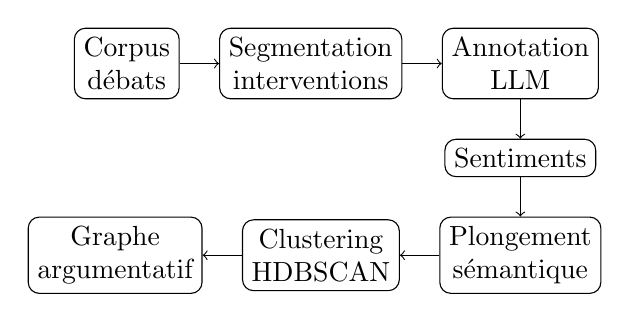
\begin{tikzpicture}[
node distance=0.5cm and .5cm,
box/.style={rectangle, draw, rounded corners, align=center}
]

\node[box] (corpus) {Corpus\\débats};

\node[box, right=of corpus] (seg) {Segmentation\\interventions};
\node[box, right=of seg] (llm) {Annotation\\LLM};

\node[box, below=of llm] (sent) {Sentiments};
\node[box, below=of sent] (embed) {Plongement\\sémantique};
\node[box, left=of embed] (cluster) {Clustering\\HDBSCAN};

\node[box, left=of cluster] (graph) {Graphe\\argumentatif};

\draw[->] (corpus) -- (seg);
\draw[->] (seg) -- (llm);
\draw[->] (llm) -- (sent);
\draw[->] (sent) -- (embed);
\draw[->] (embed) -- (cluster);
\draw[->] (cluster) -- (graph);

\end{tikzpicture}

\caption{Chaîne de traitements de structuration argumentative.}
\label{fig:pipeline}
\vspace{-.5cm}
\end{wrapfigure}

La typologie retenue s’inspire des schémas classiques de l’\textit{argument mining} distinguant \textit{claim}, \textit{premise} et unités non argumentatives \cite{lippi2016,peldszus2015}. Afin de simplifier l’annotation automatique et de mieux correspondre aux formes discursives observées dans les débats parlementaires, ces catégories ont été adaptées en quatre classes : affirmation, argument, opposition et contexte.

\begin{table}[h]
\centering
\renewcommand{\arraystretch}{1.2}
\begin{tabularx}{\linewidth}{l X X}
\toprule
Catégorie & Définition & Exemple \\
\midrule

Contexte & Une précision ou une information descriptive sans défendre ni contester une affirmation.
& La parole est à M. Marcellin Nadeau. \\

Affirmation & Un fait, une position ou une proposition.
& Il est effectivement essentiel de redresser nos comptes publics : je crois que tout le monde s'accorde là-dessus. \\

Argument & Une raison qui soutient une affirmation, présente ou implicite.
& Le risque pour l'emploi, comme en 2012, n'est pas négligeable. \\

Opposition & Une raison qui conteste une affirmation, présente ou implicite.
& C'est à cause de vous ! \\

\bottomrule
\end{tabularx}
\caption{Typologie argumentative utilisée pour l’annotation des phrases.}
\label{tab:exemples}
\end{table}

Le Tableau~\ref{tab:exemples} donne la définition de chaque catégorie ainsi qu'un exemple. Ainsi, toute l'annotation est centrée autour de la catégorie affirmation, les autres étant définies par rapport à cette dernière. La chaîne de traitements qui suit est résumée dans la Figure~\ref{fig:pipeline}.


Les débats sont d’abord segmentés en interventions correspondant à une prise de parole continue d’un locuteur sur un point de l’ordre du jour. Chaque segment est ensuite soumis à un modèle Llama 3\footnote{\url{https://huggingface.co/meta-llama/Llama-3.3-70B-Instruct}.} via un prompt contrôlé. Le modèle segmente le texte en phrases et attribue à chacune une étiquette argumentative parmi les quatre catégories définies précédemment. Ce traitement par segment, plutôt que phrase isolée, permet au modèle de prendre en compte le contexte discursif immédiat. Une vérification manuelle rapide sur un échantillon montre une qualité satisfaisante de la classification avec cette stratégie.

Cette approche repose sur une stratégie de \textit{few-shot prompting}, permettant d’obtenir une annotation argumentative de qualité acceptable sans disposer d’un corpus préalablement annoté.
Conformément aux résultats de \cite{gorur2025}, l’usage d’un modèle génératif se révèle qualitativement plus performant qu’un modèle discriminatif de type BERT \cite{devlinCLT19} pour la détection des relations argumentatives, tout en évitant une phase d’annotation supervisée.


Une analyse de sentiment est ensuite appliquée à l’aide d'un modèle RoBERTa \footnote{\url{https://huggingface.co/cardiffnlp/twitter-roberta-base-sentiment-latest}.} afin d’identifier les zones d’intensité émotionnelle. Les phrases sont chacune représentées par des plongement sémantiques. \footnote{\textit{Embeddings} générés avec paraphrase-multilingual-MiniLM-L12-v2 \\(\url{https://huggingface.co/sentence-transformers/paraphrase-multilingual-MiniLM-L12-v2)}.}

Une \textit{clusterisation} non supervisée est réalisée sur l'ensemble du corpus à l’aide de HDBSCAN, puis visualisée par réduction de dimension UMAP, afin d’identifier des regroupements thématiques au sein des catégories argumentatives. Chaque cluster est décrit automatiquement en fonction des termes utilisés et des catégories argumentatives reconnues.

Une \textit{clusterisation} non supervisée supplémentaire est appliquée afin de détecter des sous-groupes thématiques au sein de chaque catégorie argumentative. Cette étape révèle une typologie émergente des modes d’argumentation qui sera étudiée prochainement et comparée à l'état de l'art.

Enfin, un graphe de relations argumentatives est construit. Les nœuds représentent des unités argumentatives, i.e. des phrases préalablement classées, et les relations sont établies selon la proximité thématique, la
relation argumentative et la polarité émotionnelle.
La proximité thématique est établie par l'appartenance à un même cluster thématique. La relation argumentative est établie si une affirmation est suivie par une opposition ou un argument, ou si une opposition est suivie par un argument. La plausibilité est vérifiée par un modèle Llama 3 de chat via \textit{few-shot prompting} avec exemples positifs et négatifs. La polarité émotionnelle est établie si deux phrases sont reliées et une des deux au moins est intense au regard de l'analyse de sentiments.
Les acteurs parlementaires sont projetés sur ce graphe sous forme d'hyperarcs et de centroïdes en fonction des arguments mobilisés.

\section{Résultats et discussion}

\begin{wraptable}{r}{0.3\textwidth}
\centering\vspace{-.5cm}
\begin{tabular}{lc}
\hline
Catégorie & Proportion \\ 
\hline
Contexte & 43\% \\
Affirmation & 38\% \\
Opposition & 10\% \\
Argument & 9\% \\
\hline
\end{tabular}
\caption{Distribution des catégories argumentatives dans le corpus.}
\label{tab:proportion}
\vspace{-.3cm}
\end{wraptable}
La première analyse quantitative des annotations produites par le modèle montre une distribution fortement déséquilibrée des catégories argumentatives. Le Tableau~\ref{tab:proportion} donne les proportions d'apparition pour chaque catégorie. Les oppositions et les arguments apparaissent ainsi nettement sous-représentés. Cette distribution suggère que le discours parlementaire est majoritairement structuré autour de la contextualisation et de l’énonciation de positions, plutôt que par une confrontation explicite d’arguments ou d’oppositions formalisées.

La faible proportion d’oppositions semble en partie liée à une proximité sémantique et discursive avec la catégorie des affirmations, rendant parfois la frontière entre ces deux classes difficile à tracer. Cette observation souligne à la fois une limite de la typologie retenue et une piste d’amélioration méthodologique, notamment par l’introduction de sous-catégories ou de relations argumentatives plus fines.

Une évaluation manuelle réalisée sur un échantillon de phrases annotées indique un taux de validité d’environ 80\%. Ce résultat confirme la qualité globale de l’annotation automatique, tout en appelant à la prudence. Ce taux doit en effet être interprété à la lumière de la simplicité relative de la typologie utilisée et de la méthode de \textit{few-shot prompting} relativement peu robuste. Une catégorisation plus fine serait plus long à paramétrer, mais offrirait en contrepartie une richesse interprétative accrue.

L’analyse de la progression temporelle des débats ne permet pas de faire émerger de tendances claires entre les interventions successives. L’ordre des prises de parole semble avoir un impact limité sur la structure argumentative des interventions suivantes. Les discours apparaissent ainsi largement indépendants les uns des autres du point de vue de leur construction argumentative.

Cette observation est toutefois nuancée par une analyse qualitative de débats d’origine. Celle-ci montre que les réactions aux interventions précédentes sont souvent intégrées de manière subtile dans le discours suivant, sous forme d’allusions, de reformulations ou de références implicites. Par ailleurs, certaines réactions prennent la forme d’interjections ou de prises de parole brèves, lorsque la personne n'a pas la parole, qui ne sont pas toujours systématiquement retranscrites dans le jeu de données utilisé. Ces éléments expliquent en partie la faible visibilité computationnelle des relations inter-interventions.

L’analyse révèle en revanche une forte structuration argumentative interne à chaque intervention. Les arguments, affirmations et éléments de contexte s’organisent principalement à l’échelle du discours individuel. Les relations entre interventions, et plus particulièrement entre arguments portés par des locuteurs différents, apparaissent plus rares mais également plus significatives lorsqu’elles sont détectées. Ces relations constituent ainsi des points d’ancrage privilégiés pour l’analyse des dynamiques discursives du débat.

Ces résultats peuvent s’expliquer par la nature même du discours parlementaire. Les interventions sont en grande partie préparées en amont, avec parfois des réponses anticipées, mais surtout avec un souci marqué de cohérence interne. Le discours est ainsi conçu comme un objet autonome, davantage que comme une réplique immédiate à une intervention précédente. Cette caractéristique institutionnelle limite mécaniquement la visibilité des chaînes argumentatives inter-discursives.

Ces observations invitent à relativiser l’idée d’un débat parlementaire comme interaction argumentative continue, et à le considérer plutôt comme une juxtaposition de prises de position discursivement cohérentes, reliées par des points de contact ponctuels mais structurants.

Enfin, ces résultats ouvrent des perspectives méthodologiques importantes. Il serait particulièrement pertinent de tester cette approche dans des contextes discursifs moins structurés, tels que les débats en ligne, les forums politiques ou les échanges sur les réseaux sociaux. Dans ces espaces, les réactions immédiates, les confrontations explicites et les chaînes argumentatives inter-interventions sont plus fréquentes, ce qui permettrait d’évaluer plus finement la capacité de la méthode à détecter et modéliser les relations argumentatives dynamiques.

Ainsi, les résultats obtenus ne constituent pas seulement une analyse du débat parlementaire, mais également un révélateur des propriétés discursives propres à ce type d’institution, tout en soulignant l’intérêt d’étendre la méthodologie à d’autres formes d’expression politique.

Les clusters montrent une cohérence thématique significative, confirmant la pertinence de la segmentation argumentative. Certains thèmes sont principalement associés à des oppositions, tandis que d’autres sont dominés par des arguments justificatifs ou contextuels.

La projection des acteurs révèle des proximités discursives parfois indépendantes des appartenances partisanes, suggérant l’existence de styles argumentatifs transversaux. Inversement, des divergences apparaissent au sein de mêmes groupes politiques.

Cette modélisation permet ainsi de lire les débats comme une confrontation de modes d’expression et de stratégies argumentatives, et non uniquement comme une confrontation de positions politiques. Elle enrichit la compréhension des dynamiques parlementaires en révélant des dimensions discursives souvent invisibles dans les analyses traditionnelles.

\section{Perspectives}


La détection automatique des arguments et de leurs relations demeure, dans le contexte actuel, un champ scientifique riche et encore largement ouvert. Malgré les avancées récentes, la modélisation fine des structures argumentatives, en particulier dans des corpus complexes et fortement contextualisés comme les débats parlementaires, soulève encore de nombreuses questions théoriques et méthodologiques. Les résultats obtenus dans ce travail, tout comme ceux rapportés dans la littérature récente \cite{gorur2025, cabessa2025}, montrent que la qualité des annotations et des relations détectées reste perfectible, mais suffisamment robuste pour ouvrir de nouvelles pistes d’exploration.

Dans ce contexte, les grands modèles de langage apparaissent comme une méthode particulièrement efficace pour l’\textit{argument mining}, en raison de leur capacité à produire des annotations qualitatives sans nécessiter de corpus annotés, ou seulement à partir de quelques exemples. Cette propriété constitue un atout majeur pour les humanités numériques, où les ressources annotées sont souvent rares. Néanmoins, la robustesse, la stabilité et la reproductibilité de ces modèles doivent encore être évaluées de manière systématique, notamment face aux variations de corpus, de domaines et de formulations discursives.

Au-delà de la seule détection argumentative, l’enjeu principal réside dans l’articulation entre ces avancées méthodologiques et les usages concrets des documents structurés. Les systèmes de \textit{Retrieval-Augmented Generation}\cite{lewis2020}, largement mobilisés aujourd’hui, ne sont pas encore considérés comme des outils fiables d’analyse scientifique, mais plutôt comme des interfaces exploratoires permettant d’interagir en langage naturel avec des corpus documentaires. Dans ce cadre, la structuration argumentative et relationnelle des documents apparaît comme un levier essentiel pour enrichir les possibilités exploratoires offertes par ces systèmes.

Une telle structuration permet en effet de multiplier les niveaux de lecture : par thématique, par type d’argument, par relation argumentative, par tonalité émotionnelle ou encore par style discursif. Elle autorise des parcours guidés dans les corpus, favorisant une exploration raisonnée plutôt qu’une simple récupération textuelle. De plus, une recherche documentaire tenant compte de cette structuration améliore en aval la qualité des générations produites par les systèmes de RAG, en les rendant plus cohérentes, plus contextualisées et, surtout, plus explicables.

Ces perspectives invitent ainsi à concevoir la structuration des débats parlementaires non comme une fin en soi, mais comme une infrastructure interprétative au service de nouvelles formes d’exploration, de discussion et d’analyse des corpus politiques. Elles ouvrent la voie à une articulation renouvelée entre intelligence artificielle, structuration documentaire et herméneutique computationnelle, pleinement inscrite dans les objectifs des humanités numériques.

\printbibliography


\end{document}